%%%% ijcai09.tex

\typeout{IJCAI-09 Instructions for Authors}

% These are the instructions for authors for IJCAI-09.
% They are the same as the ones for IJCAI-07 with superficical wording
%   changes only.

\documentclass{article}
% The file ijcai09.sty is the style file for IJCAI-09 (same as ijcai07.sty).
\usepackage{ijcai09}

% Use the postscript times font!
\usepackage{times}
\usepackage{float}
\usepackage{graphicx}

%\usepackage{lipsum}% http://ctan.org/pkg/lipsum
%\usepackage[showframe]{geometry}% http://ctan.org/pkg/geometry


% the following package is optional:
%\usepackage{latexsym} 

% Following comment is from ijcai97-submit.tex:
% The preparation of these files was supported by Schlumberger Palo Alto
% Research, AT\&T Bell Laboratories, and Morgan Kaufmann Publishers.
% Shirley Jowell, of Morgan Kaufmann Publishers, and Peter F.
% Patel-Schneider, of AT\&T Bell Laboratories collaborated on their
% preparation.

% These instructions can be modified and used in other conferences as long
% as credit to the authors and supporting agencies is retained, this notice
% is not changed, and further modification or reuse is not restricted.
% Neither Shirley Jowell nor Peter F. Patel-Schneider can be listed as
% contacts for providing assistance without their prior permission.

% To use for other conferences, change references to files and the
% conference appropriate and use other authors, contacts, publishers, and
% organizations.
% Also change the deadline and address for returning papers and the length and
% page charge instructions.
% Put where the files are available in the appropriate places.

\title{Determining Genre of Classical Literature with Machine Learning}
\author{Ben Guthrie, Jordan Henstrom, Ben Horrocks, Ryan West \\
Department of Computer Science\\
Brigham Young University \\
CS 478, Winter 2019}

\begin{document}

\maketitle

\begin{abstract}
Text classification is a popular problem in machine learning. The ability for a program to understand classifications and distinctions between texts can be useful for a wide array of real-world applications. It was because of this that we decided to focus on teaching our learning model to classify entire books worth of text as either fiction or nonfiction. Using indicators such as word frequency and word count allowed us to approach the problem. We trained on a variety of different models. We initially found that due to possible imbalance in our data set, MLP tended to perform poorly, while Decision Trees and Ensembles of Random forests performed much better. We refined our model with testing an ensemble of our previous models. However, we found that due to the poor performance of MLP and clustering, the overall accuracy of the Ensemble we created did not perform as well as the Ensemble of Random Forests.
\end{abstract}

\section{Introduction}

Classification of literary works is significantly different from normal text classification. One big reason for this is length, as books are generally much longer than most other text mediums. Additionally, the classifications of literary works are more nuanced than other sources such as newspaper articles. This has lead to a high degree of variation in previous models of literary classification. A large part of the background information that contributed to this project comes from things that we learned throughout the semester. However, there were additional avenues beyond class materials that we explored in an effort to improve and refine our model.

\subsection{Background information}

One such avenue was the paper \textit{Genre Identification and the Compositional Effect of Genre in Literature} authored by Joseph Worsham and Jugal Kalita. This study was of interest to us in part because they used the same data set that we used. Their study focused on specific genre classification such as romance or adventure stories. Although our learner is focused more broadly on distinguishing fiction from nonfiction, it was useful to read the work of those who approached a similar topic. When discussing features, Worsham noted that using word frequencies alone is usually inadequate for the purposes of genre classification. Word frequency is defined as how many times a word appears in a section, which is in this case, an entire book. This lead to us including additional features beyond a bag of words to our model [Worsham and Kalita, 2018]. \par
We also considered a model based on predicting genre only by the title of the book. This model was created by a Github user by the name Akshay Bhatia. Like the paper by Worsham and Kalita, Bhatia’s model focused on classifying works into several genres, such as adventure and romance. However, Bhatia’s success in predicting genres solely off book titles was useful to us when we began refining our model to increase our prediction accuracy [Bhatia, 2017].


\subsection{Libraries Used}

To run our models, we used Scikit-Learn. We decided to use this model for a few reasons. First, it was an easy library to use with great documentation and examples to reference. Second, it was designed to work with NumPy and Pandas, two libraries that we worked within our project. Last, it is widely used in industry and is thought of highly. Because of this, we felt confident that it was a good choice for our models. \par
Additional libraries that we used were NumPy and Pandas. NumPy is used widely throughout most python programming. Pandas is a common library that is often used to organize data to be fed into learning algorithms. 




\section{Methods}

As we stated earlier, we focused on the classification of literary texts as either fiction or nonfiction. In this situation, we defined nonfiction as anything that purports to be nonfiction (autobiographies, biographies, textbooks, etc.). Although works like biographies and autobiographies tend to come with a lot of bias and possible embellishments, we considered them nonfiction for our purposes. We decided on this because the author viewed the works as nonfiction and therefore likely wrote them using the conventions of the genre.

\subsection{Data Source}
\begin{table*}
  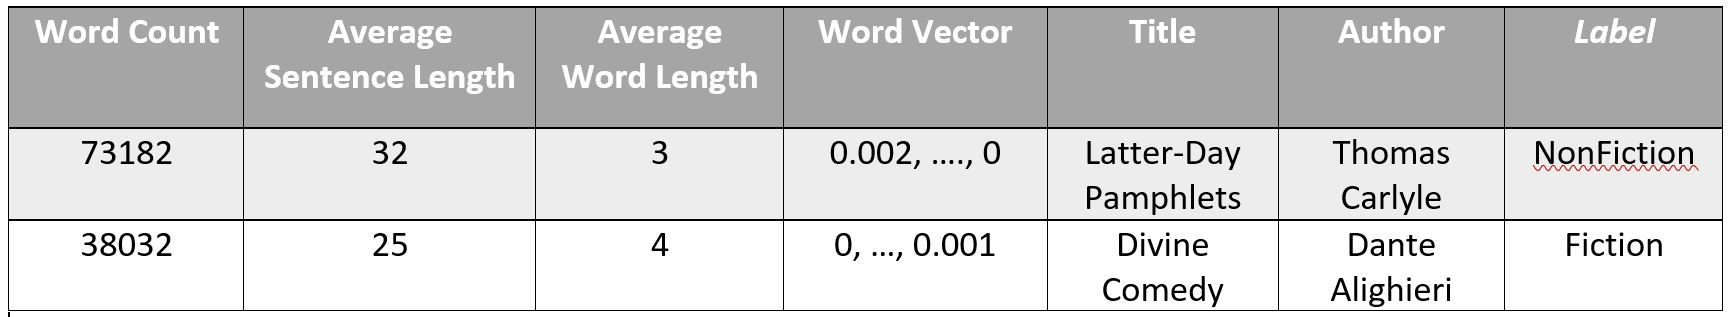
\includegraphics[width=\textwidth,height=4cm]{Table1.JPG}
  \caption{Example Rows from Data Set}
\end{table*}

The source for our data set was the online database of Project Gutenberg. This is a project aimed at making a selected count of literary classics available as free ebooks. This allowed us to quickly access hundreds of literary works to use in our model. Using a parser, we downloaded and parsed 963 instances. We then labeled each instance as either “fiction” or “nonfiction” based on Wikipedia and Goodreads. \par
There were a few hurdles that we had to address when it came to our data source. The first was that Project Gutenberg would have duplicates of some books. We didn’t quite know why this was the case, but ultimately we decided that having a few duplicates in our data set wouldn’t hurt our model’s ability to work. This is because the average scenario would be that we would have duplicates of fiction works at the same rate as those of nonfiction works. This meant that our overall data would set would have the same ratio. \par
Another problem we had was that many books would be in different languages. We decided that since we were using English words, we should disregard these entries. As a result, we did not include any works that were written in different languages. \par
The last major hurdle was that Project Gutenberg did not have their genre listed in any obvious place. This meant that for our entire data set, we had to hand label each instance as either fiction or nonfiction. This was the main reason that our data set ended up being smaller than we would have initially liked.

\subsection{Data Set}

When choosing how we wanted to construct our data set, we had to be selective in picking what we saw as the most important features in order to make up for only having roughly 1000 nodes in our data set. We used the Natural Language Toolkit (NLTK) to parse the plain text and get the number of times each of these words was used in the text, which we normalized to get a frequency value of each word in the text. After doing some preliminary research, we also decided that in addition to having a word count approach, we would also include average sentence length, word count, and average word length. We felt that these would allow our model to have a better classification accuracy.\par
We originally wanted to categorize our books into multiple genres (horror, romance, sci-fi, fantasy, mystery, and nonfiction), but when labeling our data, we found that it was difficult at times to label these books into these categories. In the end, we decided to simplify it to classification as either fiction or nonfiction. This allowed us to label data more quickly, increasing the size of our data set.\par
The largest part of our data set is word frequencies for the 1000 most common words in the English language. We chose this one because although each instance in the data set had 0’s for most of the words, we thought that the words they did have would be a good indicator of whether or not they were fiction. For example, the word ‘republican’ would be an indicator that the work is either a historical fiction centering around some governmental plot, or it is nonfiction. Since the latter is more common by far, this word could help to correctly classify the work. \par
Another feature that we used was average word length. The average length of words in the English language is four, but we didn’t know if this average held between fiction and nonfiction. It is possible that nonfiction is more pedantic than fiction and therefore will have a larger average. We didn’t know and decided it would be an interesting metric to try to see if it was indicative in any way.\par
We chose to include average sentence length for the same reason as average word length. There is no solid evidence of a correlation in sentence length and genre. However, this could have been a feature that when paired with another, gives us an idea on its genre.\par
Our last feature was how many words appeared in the book. This metric allowed for multiples of the same word, so it was merely a measurement of length. We concluded that this would be a useful metric if either fiction or nonfiction works were generally longer than the other. In that case, this feature would likely have a strong correlation to the genre of the book.

\subsection{Selected Models}

We selected five models to use as trial learning algorithms for our data: a multi-layer perceptron, a clustering algorithm utilizing nearest centroid clustering, a decision tree, logistic regression, and an ensemble of Random Forest classifiers. Although other algorithms like k-nearest neighbor and naive bayes were considered for our initial runs, we thought that sticking to a small number for our initial results would be better.\par
We decided that using an MLP learner would be a good idea because of how many features we had. Using an MLP would allow our model to filter out features that were not important for prediction. Additionally, this was the algorithm that we all had the most experience because of the extended lab we completed in class. \par
We also decided to try using a clustering algorithm because they tend to lend themselves well when things of the same classification are similar in the content. That is to say that an assumption that we made is that nonfiction books are similar to other nonfiction books, and the same is true for fiction books. This is a pretty big assumption. However, by including the learner we were able to test this idea.\par
The third model that we used was a decision tree. This model would work well if there were certain words that had a large effect on the genre. In order to use this algorithm, we had to be able to divide the feature values into nominal buckets, but luckily the Python library we used, Scikit-Learn, was able to do this quite well. \par
We then tried using logistic regression to see if that approach would improve accuracy. This model also did quite well with a slightly higher average accuracy than with the decision tree. However, there was also significantly more variation with this model than with the others. \par
The last model that we initially tried was an ensemble of random forests. We used this one largely because we wanted to include an ensemble as one of our models, and random forests are essentially collections of Decision Trees. This allowed us to explore something that we didn’t cover intensively in class.

\section{Initial Results}

The initial results using our multilayer perceptron implementation were about 80\%. But upon further inspection, we noticed that the algorithm was only ever guessing fiction. Because our data was weighted heavily toward fiction literature,  the MLP learned that always guessing fiction produced the best results for the data, and in reality learned nothing. Furthermore, the weights never converged consistently; the weighted values after training were more or less random. \textbf{Table 2} shows the best hyperparameters that we used for the initial MLP.

\begin{table}[b]
  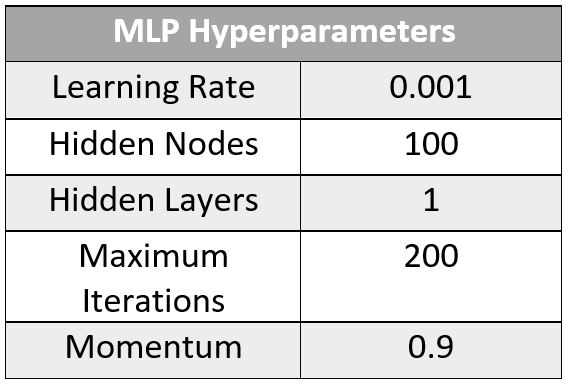
\includegraphics[width=8.5cm,height=5.5cm]{Table2.JPG}
  \caption{Hyperparameters for initial MLP}
\end{table}

\section{Refinement}

\subsection{Feature and Data Improvements}

To improve our algorithms, we first tried obtaining more data. We realized that having around 20\% of 360 instances being nonfiction gave us very few instances for our learning algorithms to learn on, so we downloaded and labeled more book texts. Because not all of the data was English, we ended up with a total of 963 Instances, with approximately 40\% of the data being nonfiction. \par
Originally our feature set was composed of the word count, average word length, average letters per word, and the frequency of the 1000 most common English words. After reviewing similar studies of genre classification, we found a study classifying book genres based on only the title and author of the text. No other context was given. We already had this data in our data set, but we were not using it in training any of our models. We decided to split our one data set into two data sets trained by two separate models. The corpus data set contains the word count, average word length, average letters per word, and the frequency of the 1000 most common English words. The title and author dataset contain the title and author of each piece of literature.

\subsection{Model Improvements}

Our initial model was an MLP that did not truly learn during the training process. For a better idea of what models worked well with our genre classification problem, we decided to try out a number of models on our original data set. \par
\begin{figure}[b]
  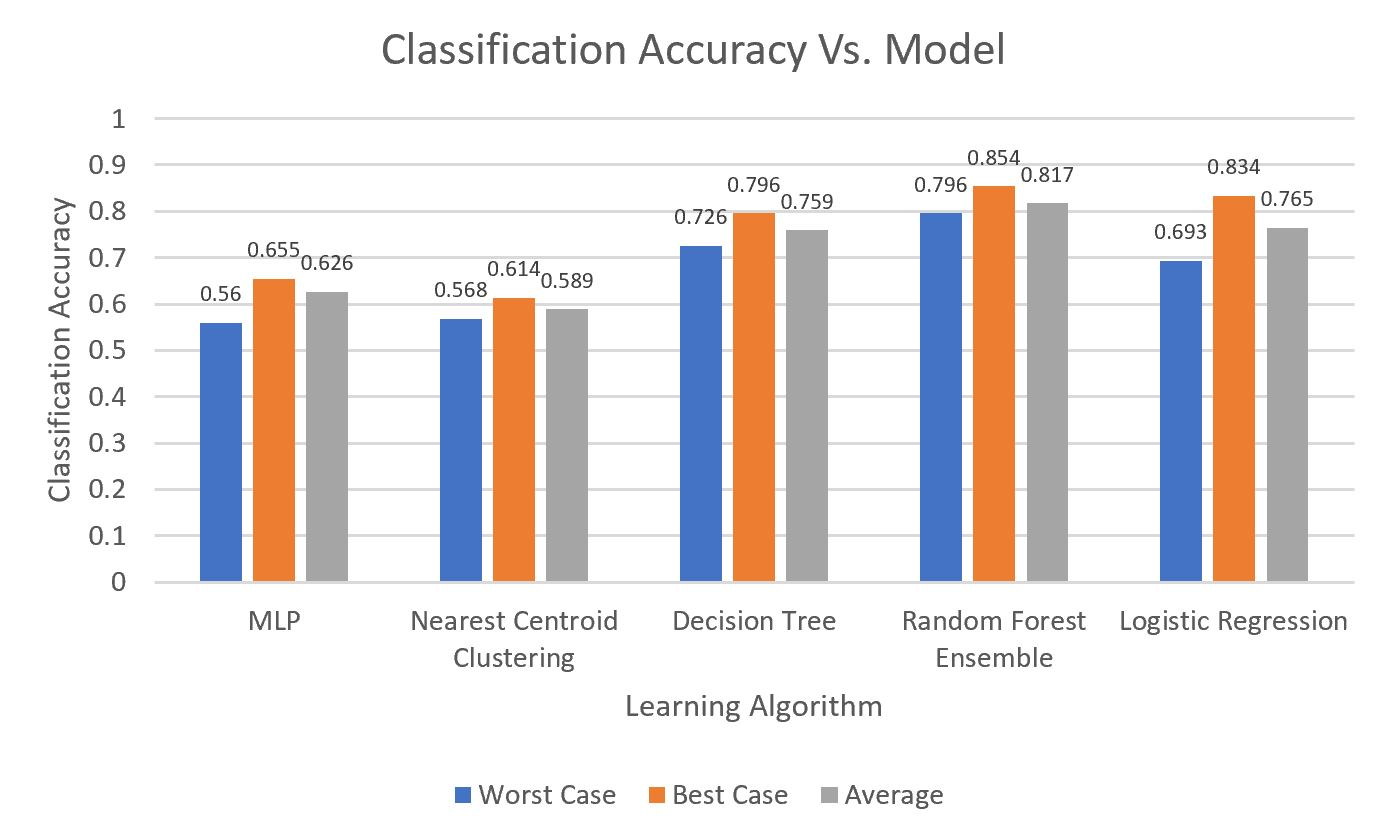
\includegraphics[width=8.5cm,height=6cm]{Figure1.JPG}
  \caption{Classification Accuracy of Several Learners}
\end{figure}
\begin{table}
  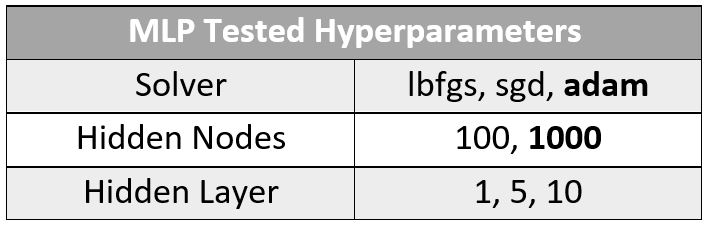
\includegraphics[width=8.5cm,height=2.8cm]{Table3.JPG}
  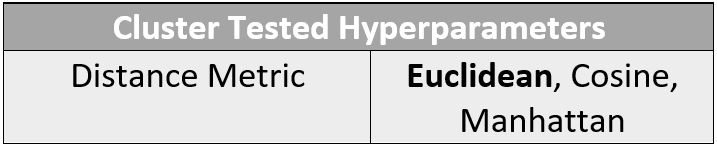
\includegraphics[width=8.5cm,height=2cm]{Table4.JPG}
  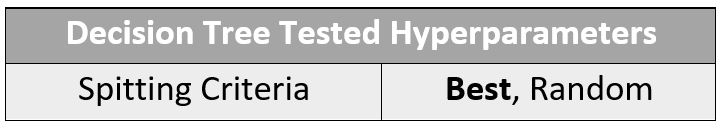
\includegraphics[width=8.5cm,height=1.5cm]{Table5.JPG}
  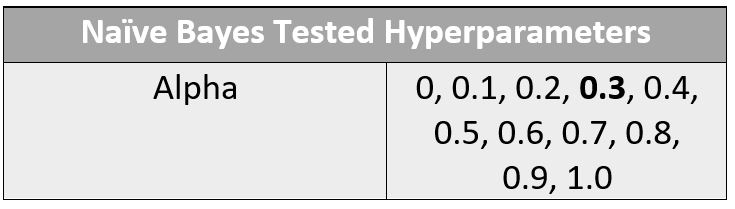
\includegraphics[width=8.5cm,height=2cm]{Table6.JPG}
  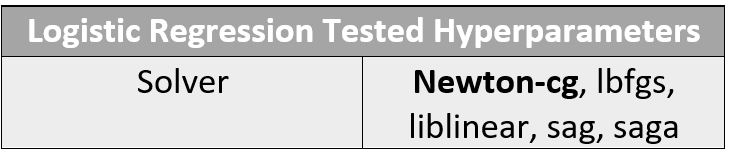
\includegraphics[width=8.5cm,height=2cm]{Table7.JPG}
  \caption{Hyperparameters for different learners}
\end{table}
\begin{figure}
  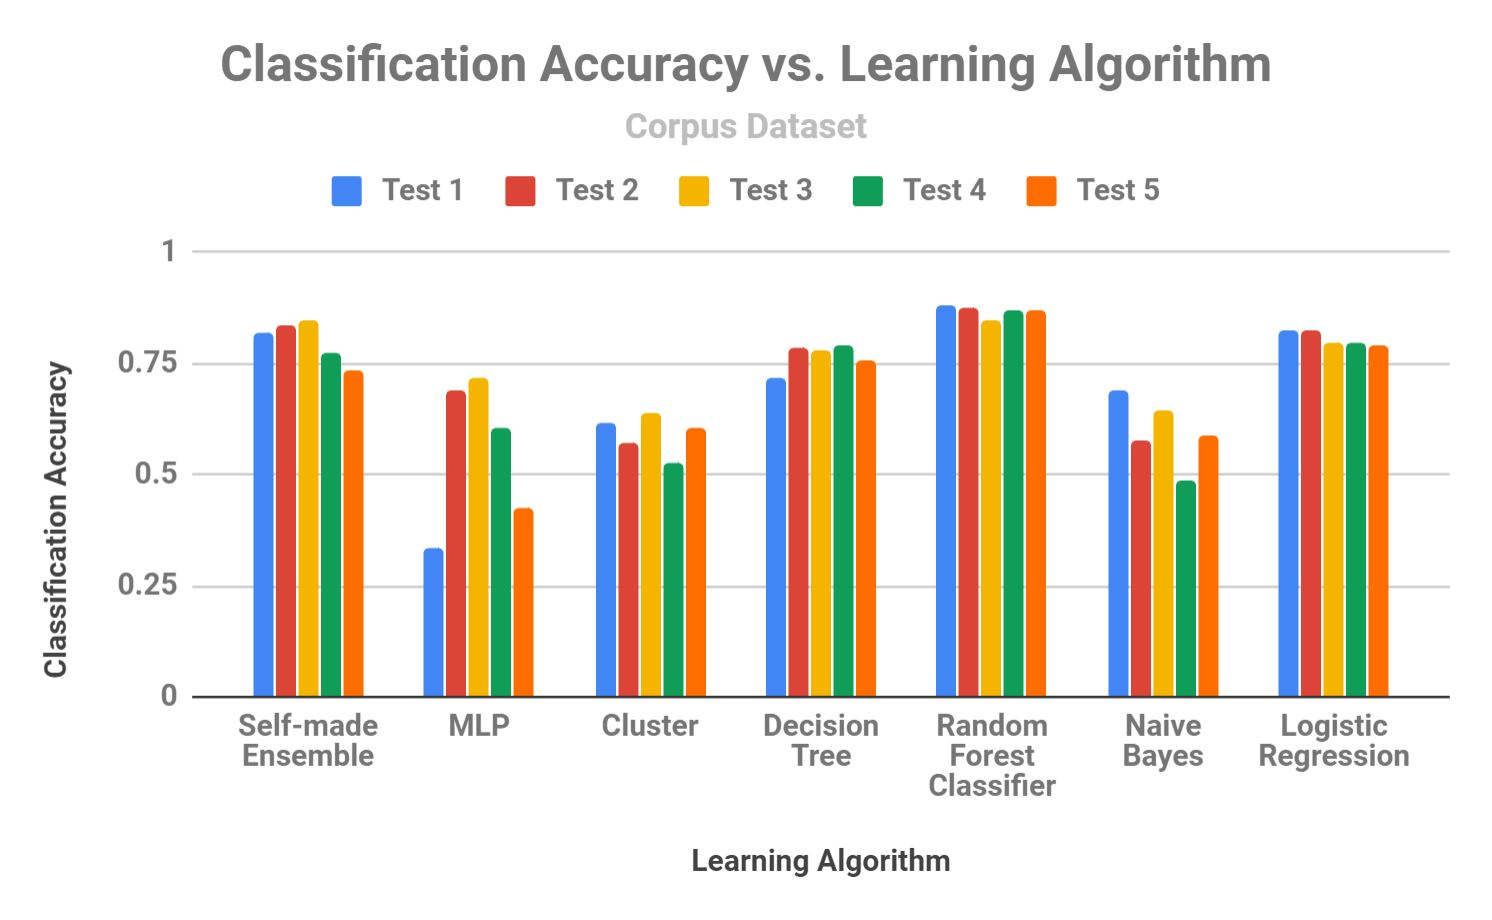
\includegraphics[width=8.5cm,height=6cm]{Figure2.JPG}
  \caption{Classification Accuracy for self-made ensemble compared to others on Corpus Dataset}
\end{figure}
\textbf{Figure 1} is a graph of classification accuracy versus each of the learning algorithms we tested in our first iteration of model improvement. We tested the original MLP, a nearest centroid clustering model, a decision tree, a random forest classifier ensemble, and a logistic regression model. The random forest classifier had an average of 81\% accuracy and relatively low variance. The second highest average accuracy was logistic regression, though the variance was higher than the other models. The decision tree had a high average and low variance compared to logistic regression. \par
	At this point, we created a split in our data set to train against the title author dataset. We trained both datasets with a variety of models. As we were testing out various models for our datasets, we also leveraged a cross-validation grid search to fine-tune the hyperparameters for each of the models we were training. \textbf{Table 3} show the hyperparameters we tested for each model. The best hyperparameter is bolded. \par
Using the optimal hyperparameters found for each model we were testing, we tested both the corpus dataset and the title and author dataset again each of these models, including the naive bayes and logistic regression models. The first one that we tested was the cropus dataset. From five tests, the top three learning models at generalizing genre classification were the decision tree, random forest classifier, and logistic regression. Shown in \textbf{Figure 2}, the random forest classifier consistently had around 80\% accuracy, while logistic regression and decision tree sat between 70\% and 75\% accuracy.\par

\begin{figure}
  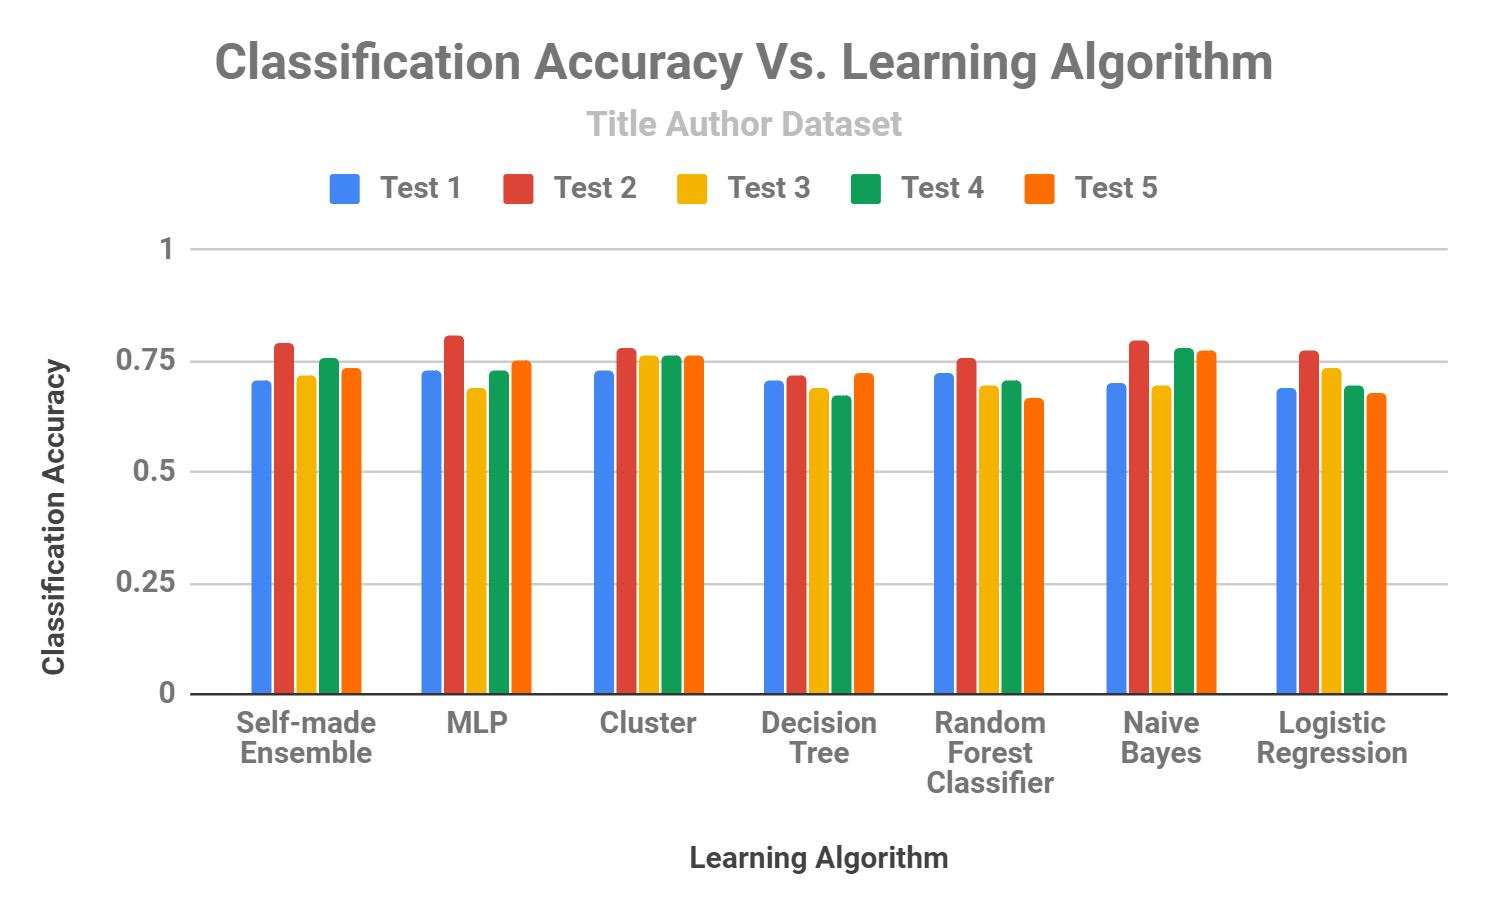
\includegraphics[width=8.5cm,height=6cm]{Figure3.JPG}
  \caption{Classification Accuracy for self-made ensemble compared to others on Title and Author Dataset}
\end{figure}

The second that we tested was the title and author dataset. For five tests, the top three learning models at generalizing genre classification based on only the title and author of the literature were an ensemble made of one of each of the other models in the test, the clustering model, and the decision tree. These three models consistently generalized with an accuracy of around 75\% while the rest sat around 70\%, shown in \textbf{Figure 3}. 
Our final models were two ensembles based on the top three learning models for each dataset which voted based on the majority class.

\section{Final Results}

The final results that we had on the corpus dataset can be seen in \textbf{Figure 4}. The corpus dataset ensemble is made of a decision tree, a random forest classifier, and a logistic regression model. The random forest classifier consistently predicted with 80\% accuracy while the decision tree and the logistic regression model were between 70\% and 75\%. \par
The complete corpus ensemble predicted the genre with an accuracy of 75\%. Unfortunately, the ensemble does not predict at a much higher accuracy than the random forest classifier. We believe that the decision tree and logistic regression may learn similar important telling aspects of the corpus dataset different from those of the random forest classifier, so their two votes override the possibly correct vote of the random forest classifier that is more accurate. \par
The final results that we had on the title and author dataset can be seen in \textbf{Figure 5}. The title and author ensemble is made of an ensemble of one of each of the originally tested models, a clustering model, and a decision tree model. All three of these models accurately predicted the genre based on only the author and title and no other context 75\% of the time. \par
Together in an ensemble, these three models voting based on the majority class, the classification accuracy was still 75\%. This may be indicative that each model was learning the same telling aspects of the title and author and an ensemble of the three was just all three voting unanimously with 75\% accuracy.
\begin{figure}
  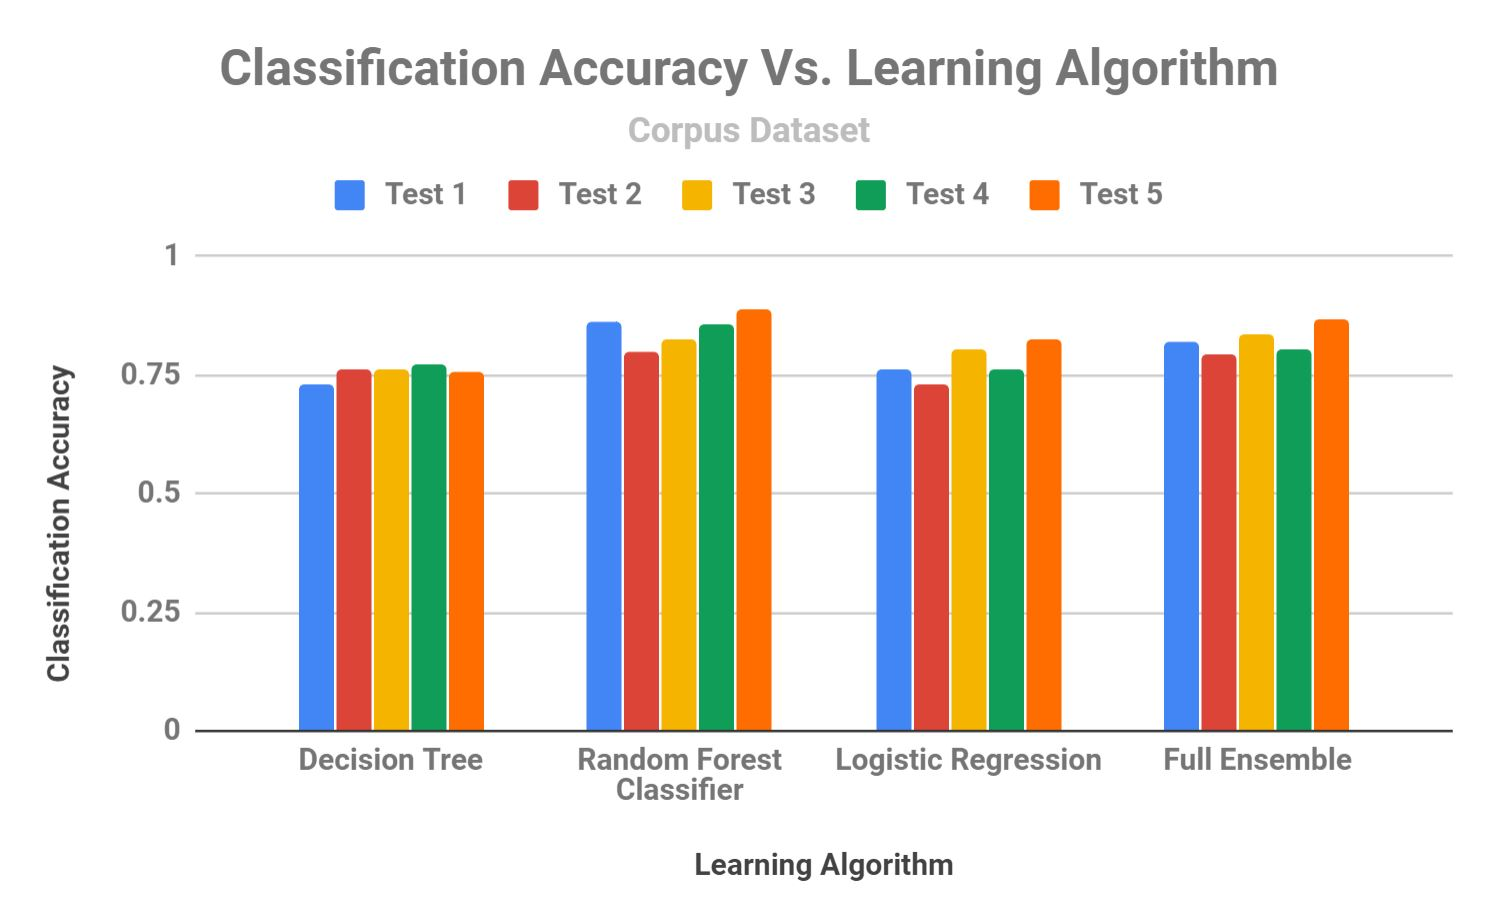
\includegraphics[width=8.5cm,height=6cm]{Figure4.JPG}
  \caption{Classification Accuracy of full ensemble on Corpus Dataset}
\end{figure}
\begin{figure}
  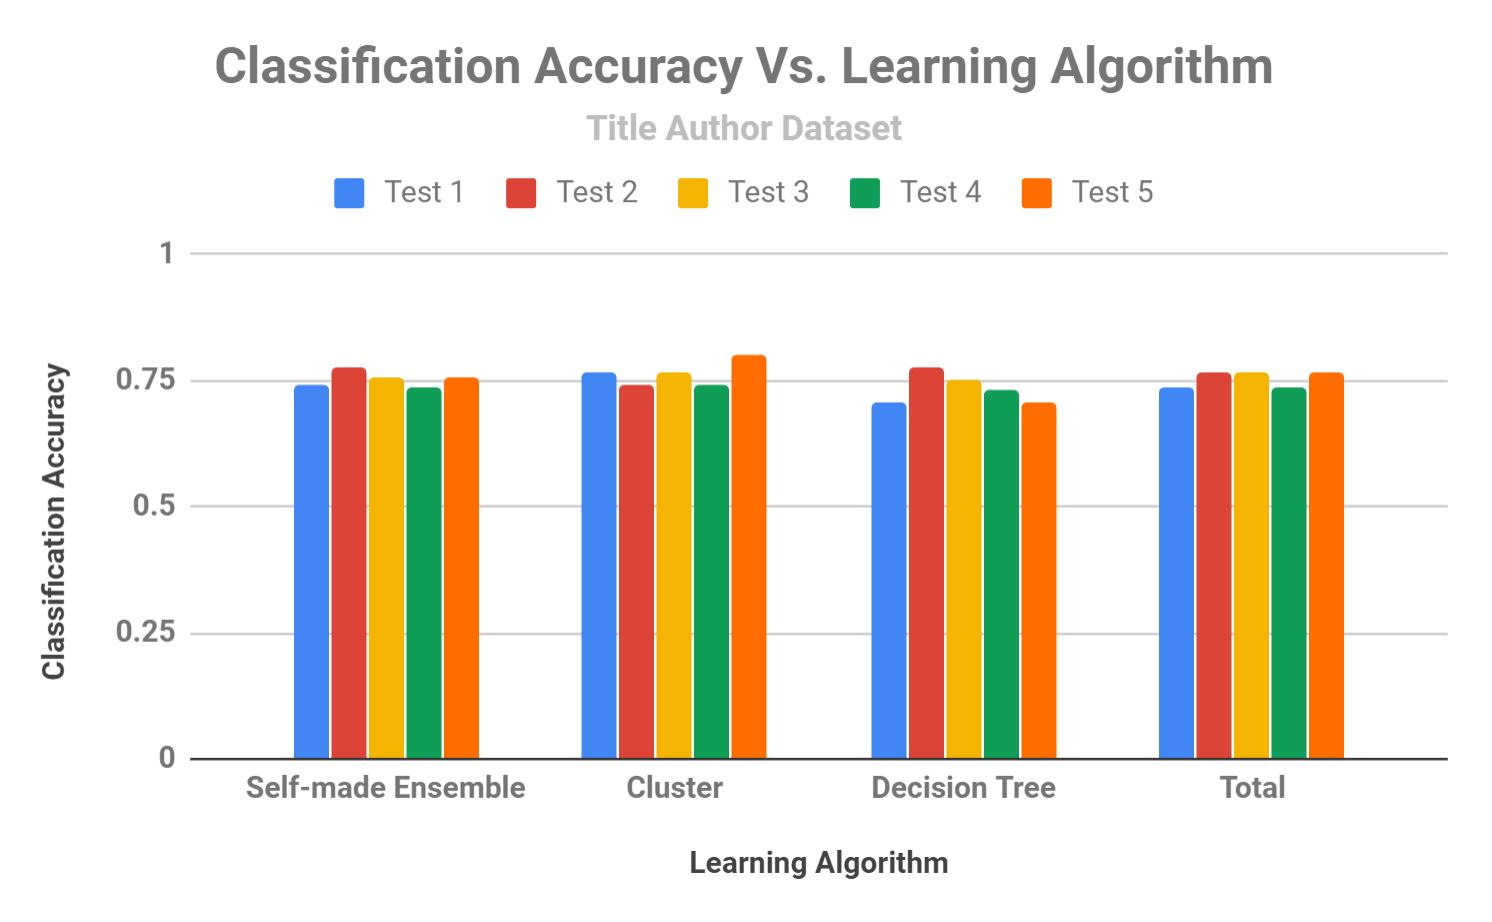
\includegraphics[width=8.5cm,height=6cm]{Figure5.JPG}
  \caption{Classification Accuracy of full ensemble on Title and Author Dataset}
\end{figure}
\section{Conclusions}

Our model showed a lot of promise. Among the benefits of our model was that it performed significantly better than either guessing or giving the majority case. Additionally, we found that this classification problem is was best solved by using an ensemble approach. Specifically this was an ensemble of random forest classifiers. The last benefit that we saw with our model was that the ensemble that we constructed using our other models had a lower likelihood to overfit. This was because, by using different models like MLP and Decision tree, we increased the chance that the ensemble would learn more parts of the data that each individual model may not learn easily.\par
Some limitations of our models were as follows: First, it is possible that our self-made ensemble might have weighted weak learners to strongly, decreasing its overall accuracy. Second, our data set could use additional refinement. More cases and more diverse features are important in increasing classification accuracy. Finally, our approach placed too much weight on the Bag of Words method. Although our background information did talk about not doing so, we did end up spending most of our time and resources on using the bag of words.

\section{Future Work}

One possible area of future work is to find another dataset to train a third ensemble on and create one grand ensemble of the two we’ve discussed and this third ensemble. This ensemble would have three estimators that were trained on three very different data sets and would predict based on three different understandings of genre.\par
There were several things that we thought could be useful as future refinement, but that would have required significant changes to our data set. The main one would have been the incorporation of SpaCy.\par
	SpaCy is a library for creating word vectors. Word vectors are lists of numbers that are used to represent a word’s attributes. This allows for a numerical representation of a word that allows someone to treat them more like continuous values. This is applicable to our models because working with continuous values opens new ways we can try to learn with them [Ahire, 2018].\par
	A possible model that we thought of to use SpaCy for is one that is based off of sentences. SpaCy helps represent context of a words in sentences, so it would be interesting to have a dataset that is just a large amount of sentences that were classified as either fictions or nonfiction. Then when we have a new book. We classify each sentence as nonfiction or fiction through our learner. This is useful because you can make a prediction on the book’s genre based on if it has more nonfiction or fiction sentences. But you can also output a percentage of the book that is fiction. This could be useful in classifying which parts of certain nonfiction books are embellishment and hyperbole.\par

\begin{thebibliography}{9}
\bibitem{Worsham} 
Joseph Worsham, Jugal Kalita
\textit{Genre Identification and the Compositional Effect of Genre in Literature}. 
University of Colorado, Colorado Springs, 2018.

\bibitem{Reeve} 
Jonathan Reeve
\textit{A Project Gutenberg Database for Text Mining}. 
Corpora, June 23, 2017.

\bibitem{Gutenberg} 
Gutenberg Database
\underline{gutenberg.org}. 
December, 1971 (2004)

\bibitem{NLTK} 
Natural Language Toolkit Platform
\underline{nltk.org}. 
2001

\bibitem{SpaCy} 
Jayesh Bapu Ahire
\textit{Introduction to Word Vectors}. 
SpaCy, March 12, 2018

\bibitem{Bhatia} 
Akshay Bhatia
\underline{github.com/akshaybhatia10/Book-Genre-Classification}. 
2017

 
\end{thebibliography}

\end{document}

